\subsection{Setup initial}

Toute cette partie est couverte par la formation précédente. Normalement, à la suite de tutoriel, vous devriez avoir obtenu le site suivant en vous rendant sur \url{http://lurlquevousavezchoisie}:\footnote{\underline{PS:}n'oubliez pas de lancer \verb|sail up -d| et \verb|sail npm run dev| si cela n'est pas déjà fait! Ne vous inquiétez pas, l'explication pour la deuxième commande va bientôt arriver\ldots}.

\begin{figure}[!h]
    \centering
    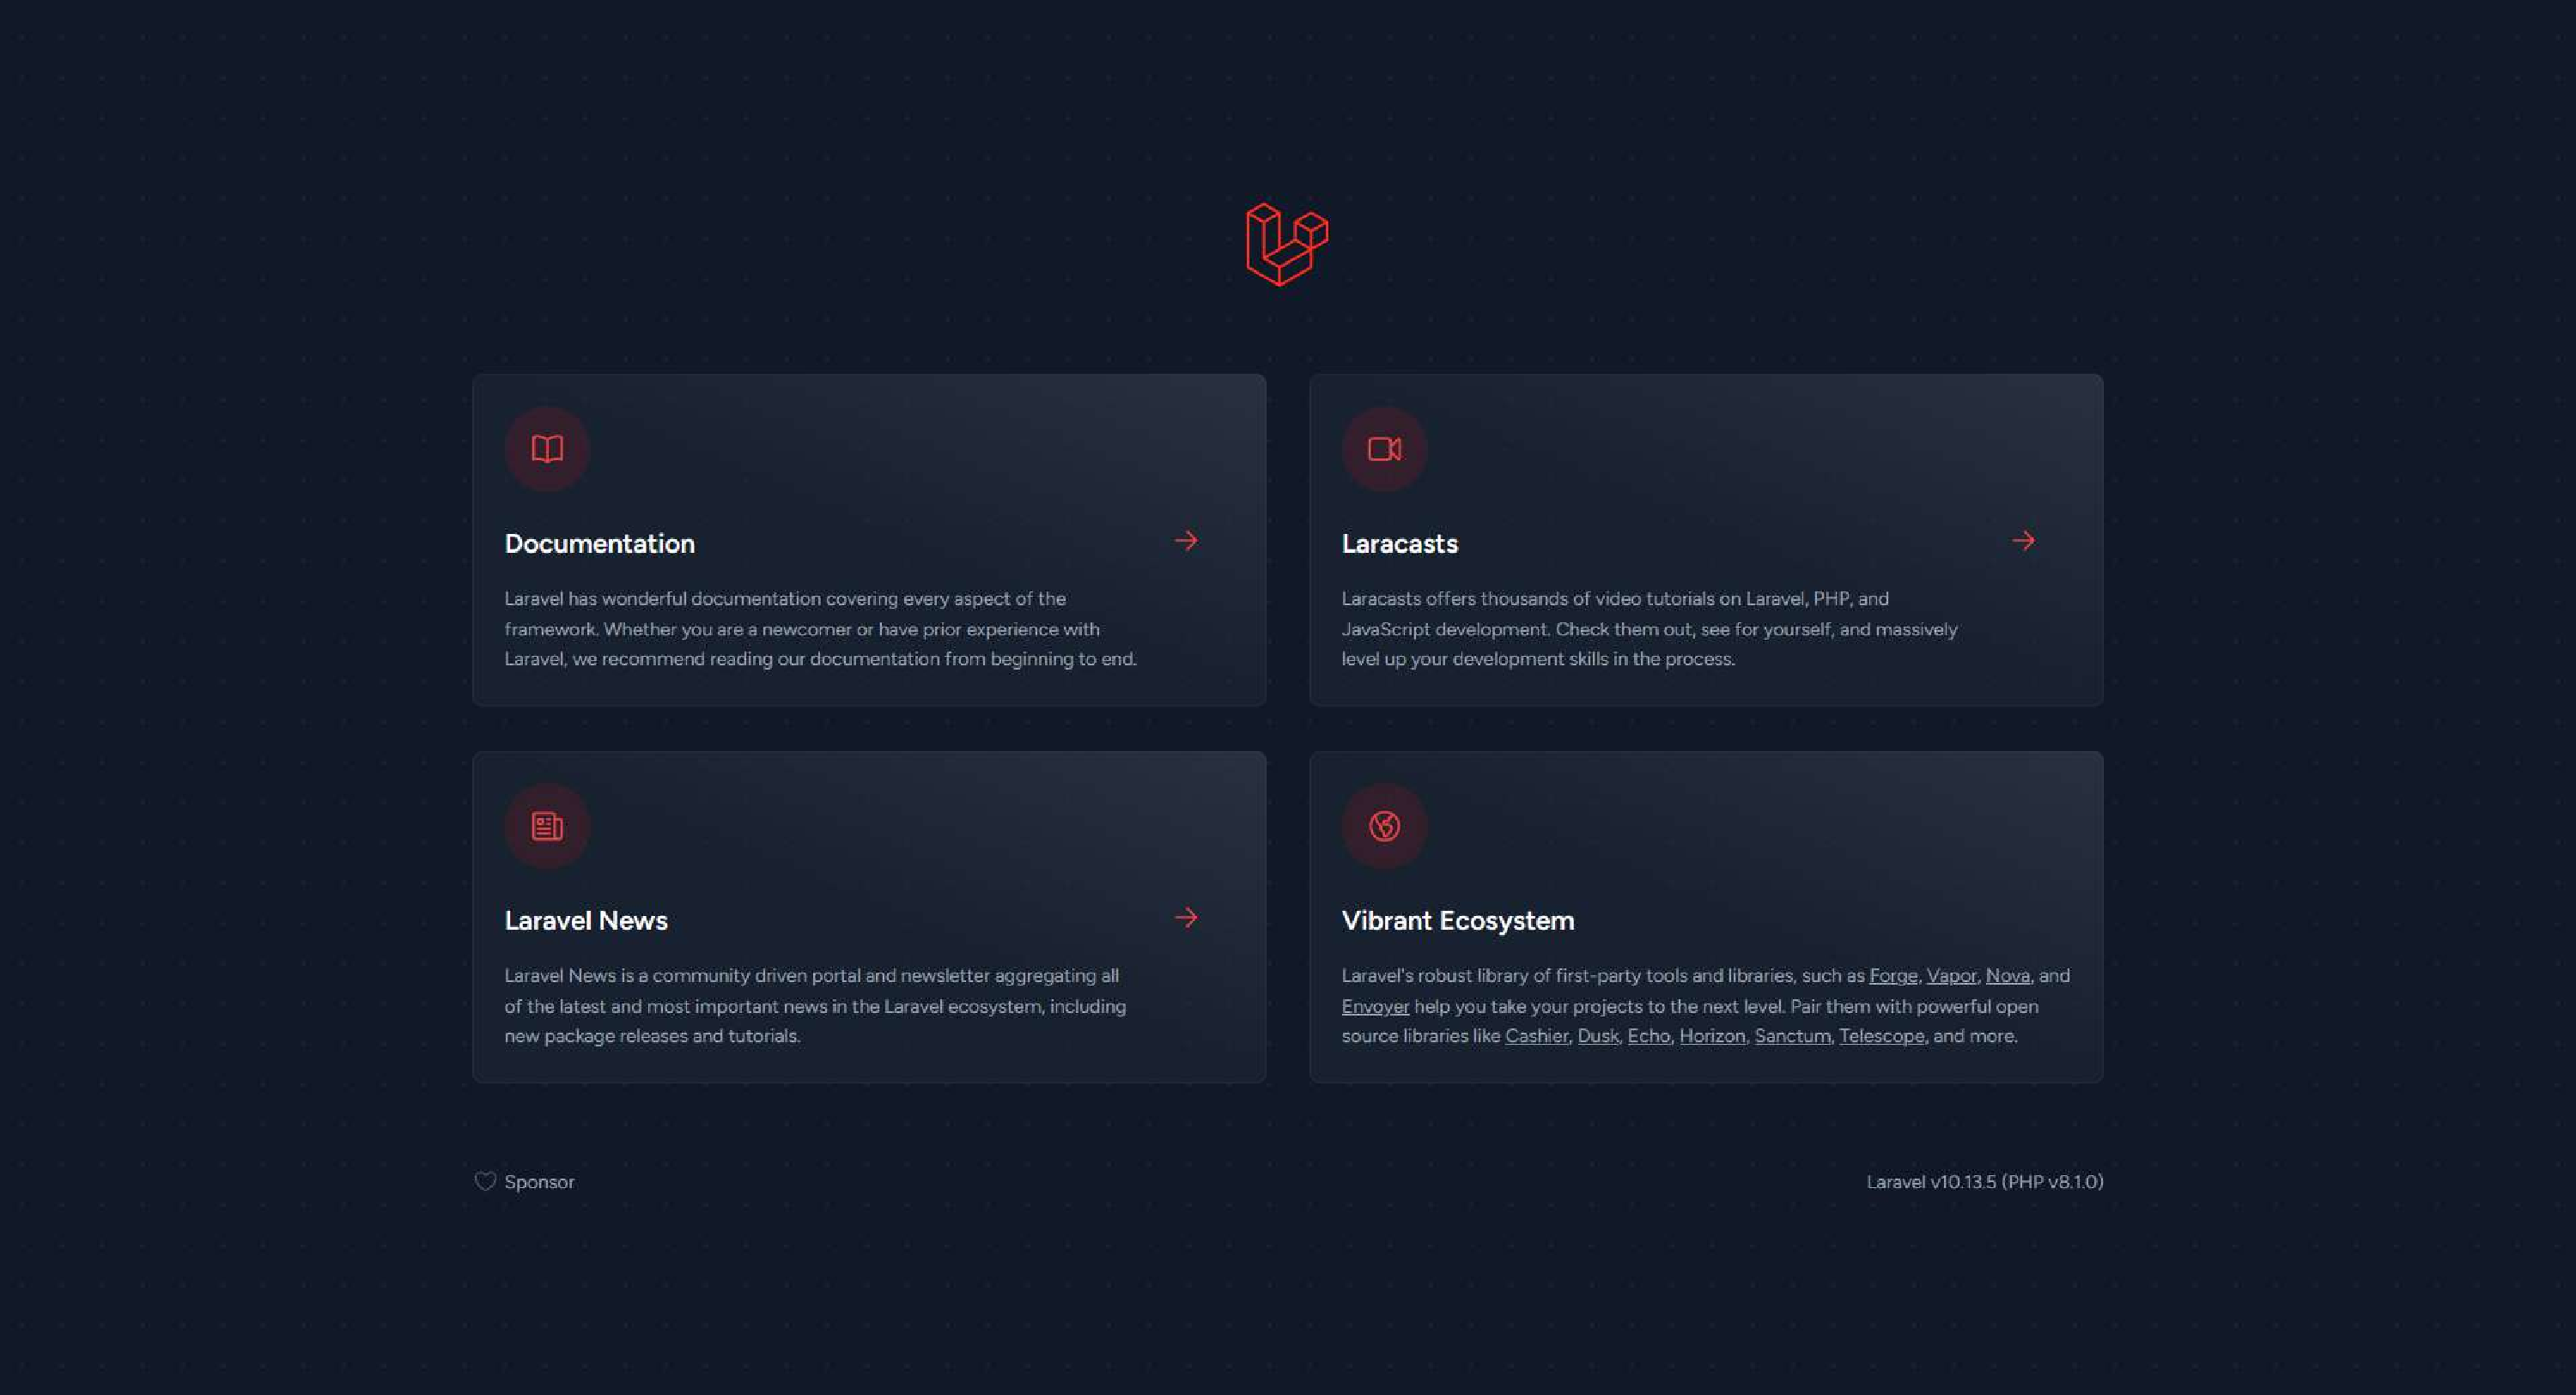
\includegraphics[width=0.75\textwidth]{figures-C1/laravel_default_website.pdf}
\end{figure}

Nous allons partir de ce site là. Pour ce tutoriel, mon projet sera appellé \texttt{tutorialstepbystep} donc son URL sera \url{http://tutorialstepbystep/}.

\newpage
\subsubsection[Extensions]{Extensions}

Vous allez rapidement remarqué de nouvelles fonctionnalités que mon IDE\footnote{Au cas où ça ne serait toujours pas clair, utilisez \vscode{} !!} possède par rapport au vôtre. Ces fonctionnalités sont rajoutées grâce aux extensions de \vscode{}. Pour installer des extensions, il vous suffit de vous rendre dans l'onglet \verb|Extensions| dans la barre d'outils à gauche de \vscode{} et d'installer celles que vous voulez.

Voici une liste non-exhaustive d'extensions utiles pour le développement web avec \laravel{} et les outils que nous utilisons:

\begin{AutoMultiColItemize}
    \item \extension{Auto Rename Tag}{Jun Han}
    \item \extension{Bootstrap 5 Quick Snippets}{Anbuselvan Rocky}
    \item \extension{CSS Peek}{Pranay Prakash}
    \item \extension{DotENV}{mikestead}
    \item \extension{HTML CSS Support}{ecmel}
    \item \extension{Image preview}{Kiss Tamas}
    \item \extension{IntelliSense for CSS class names in HTML}{Zignd}
    \item \extension{Laravel Artisan}{Ryan Naddy}
    \item \extension{Laravel Blade Component Support}{webdevsavvy}
    \item \extension{Laravel Blade formatter}{Shuhei Hayashibara}
    \item \extension{Laravel Blade Snippets}{Winnie Lin}
    \item \extension{Laravel Blade Spacer}{Austen Cameron}
    \item \extension{Laravel Extra Intellisence}{amir}
    \item \extension{Laravel goto view}{codingyu}
    \item \extension{laravel-blade}{Christian Howe}
    \item \extension{laravel-goto-components}{naoray}
    \item \extension{Material Icon Theme}{Philipp Kief}
    \item \extension{npm intellisence}{Christian Kohler}
    \item \extension{PHP Debug}{Xdebug}
    \item \extension{PHP Intelephense}{Ben Mewburn}
    \item \extension{PHP Namespace Resolver}{Mehedi Hassan}
    \item \extension{PHPStorm Parameter Hints in VScode}{MrChetan}
    \item \extension{SCSS Formatter}{Sibiraj}
\end{AutoMultiColItemize}